\documentclass[twocolumn]{article}
\usepackage{graphicx}
\usepackage{amsmath}
\usepackage{bm}
\usepackage{latexsym}
\usepackage[small]{caption}
\usepackage{hyperref}
\parskip=0pt
\setlength{\topmargin}{-18mm}
\setlength{\textheight}{240mm}

\usepackage[table]{xcolor}
\usepackage[style=nature,sorting=none,backend=biber,isbn=false,date=year,doi=false,url=true]{biblatex}
% \usepackage[
% backend=biber,
% style=alphabetic,
% citestyle=authoryear
% ]{biblatex}
 \DeclareFieldFormat{labelnumberwidth}{\mkbibbrackets{#1}}

\addbibresource{library.bib} %Imports bibliography file


\begin{document}

\twocolumn[
\begin{center}



\textbf{\Large
%Title of the paper:
Towards a fiber coupled organic molecule as a single-photon source
}
\vspace{2mm}

{

% Please list the names of the authors here,
%with the name of the presenting author in underlined.
% Use superscripts as needed to indicate which address belongs to which author.
% Do not use empty blank lines within the author/address part
%(this will result in an error).
\textbf{\underline{V. Bushmakin}$^{1,2}$, G. Stein$^1$, Y. Wang$^1$, J. Wrachtrup$^{1,2}$, A. Schell and I. Gerhardt$^{1,2}$}

\textit{$^1$3. Physikalisches Institut, Universit\"at Stuttgart and Stuttgart Research Center of Photonic Engineering (SCoPE)
and IQST, Pfaffenwaldring 57, Stuttgart 70569, Germany}\\
\textit{$^2$Max Planck Institute for Solid State Research, Heisenbergstra{\ss}e 1, 70569 Stuttgart, Germany}





%Include the email address of the corresponding author here.
e-mail: \textit{bushmakinvls@gmail.com}

}
\end{center}
]

\thispagestyle{empty}

%This is the main body of the text of the abstract.
A single-photon source is an essential tool for the developing field of quantum
technologies. Ideally, it should be spectraly compatible with other photonic devices
while providing a high flux of narrow-band photons. The single organic dye molecule
dibenzanthantherene (DBATT) embedded into a n-tetradecane Spol'skii matrix under
cryogenic conditions possesses the given characteristics, thus constitutes a
prominent single-photon source \cite{PRX}. Nevertheless, the implementation of such a
single-photon source requires a complex experimental setup involving a cryostat
with a confocal microscope for the effective collection of the molecule's emission.
Another approach is to use a single emitter coupled to an optical fiber. This
approach has the potential to transfer a single-photon source from a proof-of-
principle type of setup to a scalable “plug and play” device.
Here we present the first steps towards the fiber-coupled organic molecule single-
photon source. To conveniently couple the molecules to the fiber the solution of the
DBATT molecule in the a n-tetradecane was deposited inside a glass capillary. The
fiber end was immersed inside the capillary to collect the molecule emission. This
simplistic approach already enabled the detection of single molecules and collection
of up to 40 thousands photons per second with anti-bunching at zero reaching the
value of 0.35 \cite{PRA}. Nonetheless, the obtained emission is significantly influenced by the
Raman scattering inside the fiber. The spectrum of the molecule was filtered to
minimize the presence of the Raman scattered light in the emission of the molecule.
However, spectral filtering cuts off 70 \% of the molecular emission. Additionally, a
time filtering in the pulsed excitation scheme is examined, which holds a promise to
avoid the disadvantages introduced by the spectral filtering.
 
 
\vspace{0em}


\begin{figure}[h]
\center{
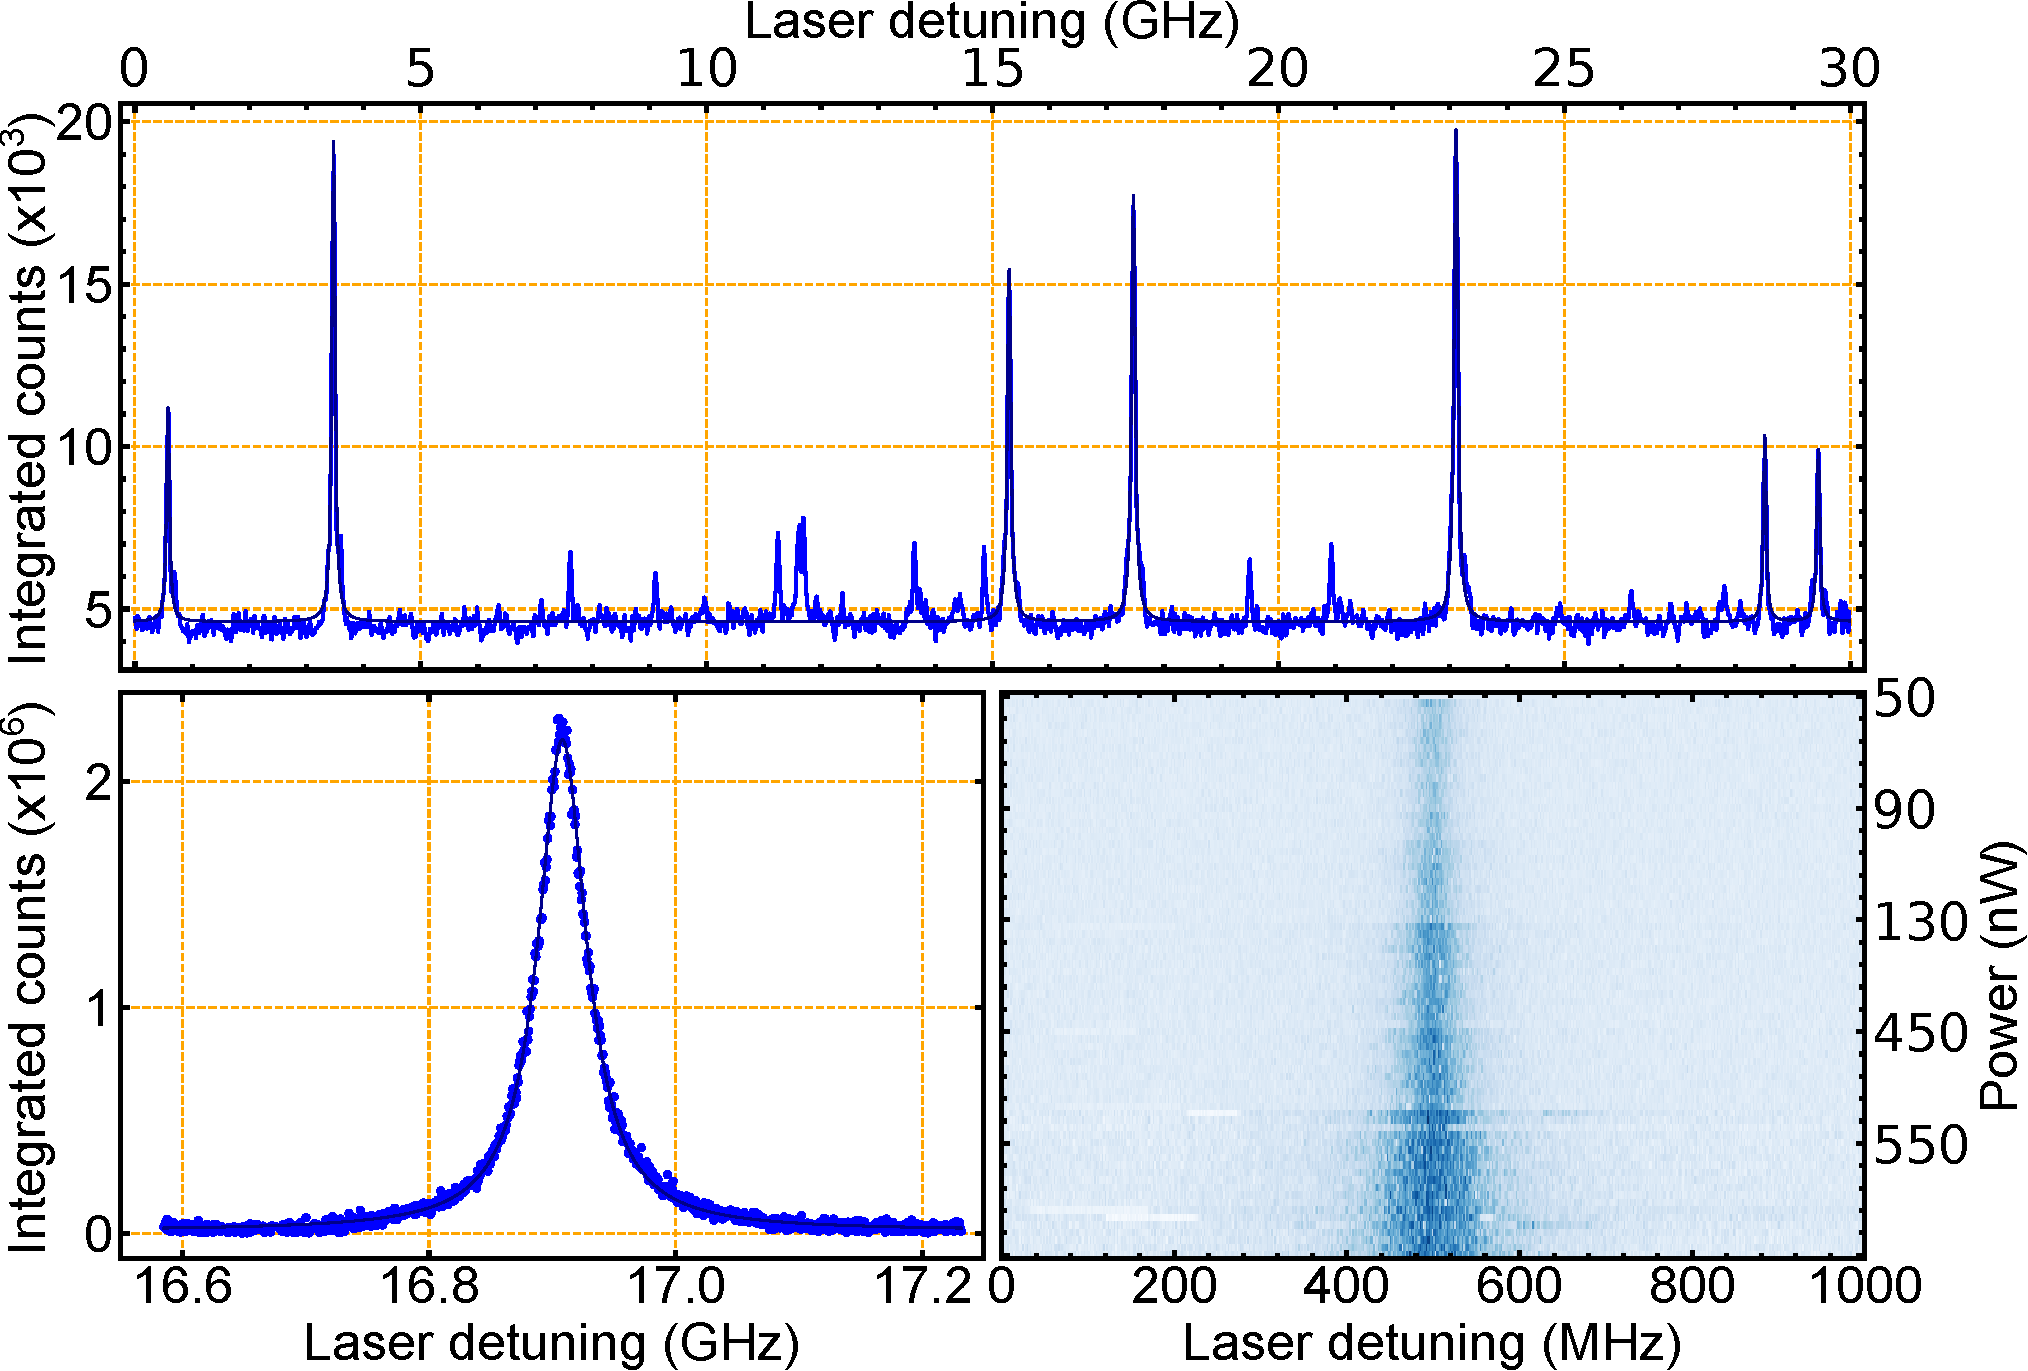
\includegraphics[width=1.\linewidth]{images/number3.pdf}

\caption{The detected with a fiber single DBATT molecules.\label{fig: molecules}}}
\end{figure}

\begin{figure}[h]
\centering
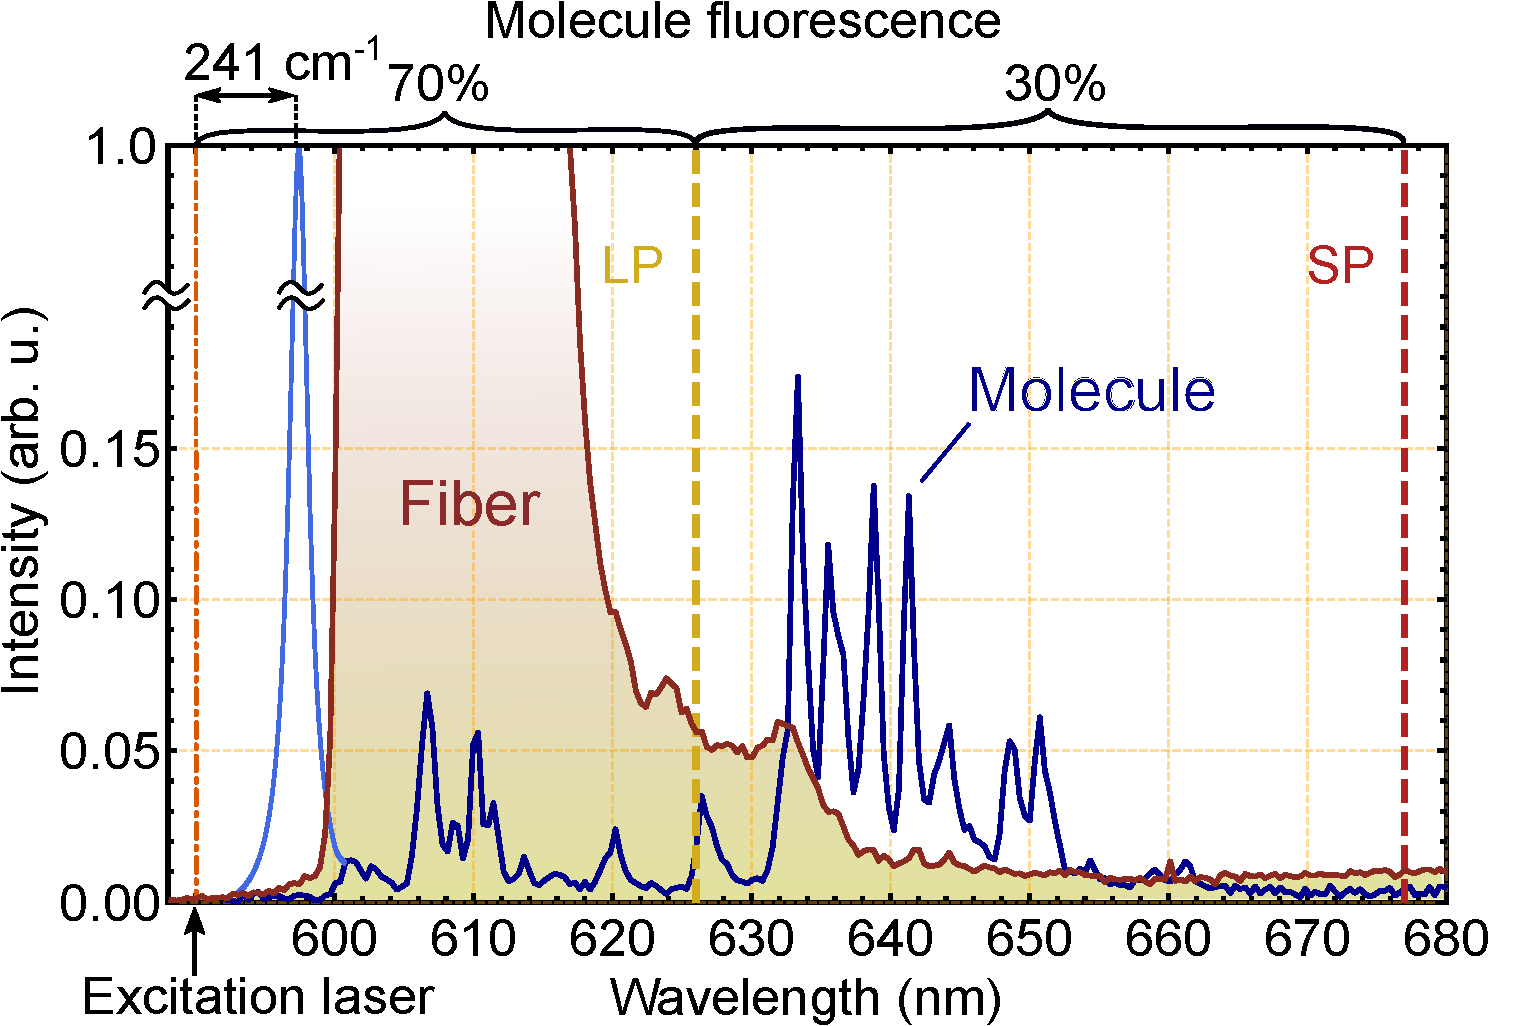
\includegraphics[width=1.\linewidth]{images/spectrum_corrected.pdf}

\caption{The spectral picture of the emission og the DBATT molecule coupled to the fiber.\label{fig: signal}}
\end{figure}

\newpage
\renewcommand{\refname}{}
\printbibliography

\end{document}